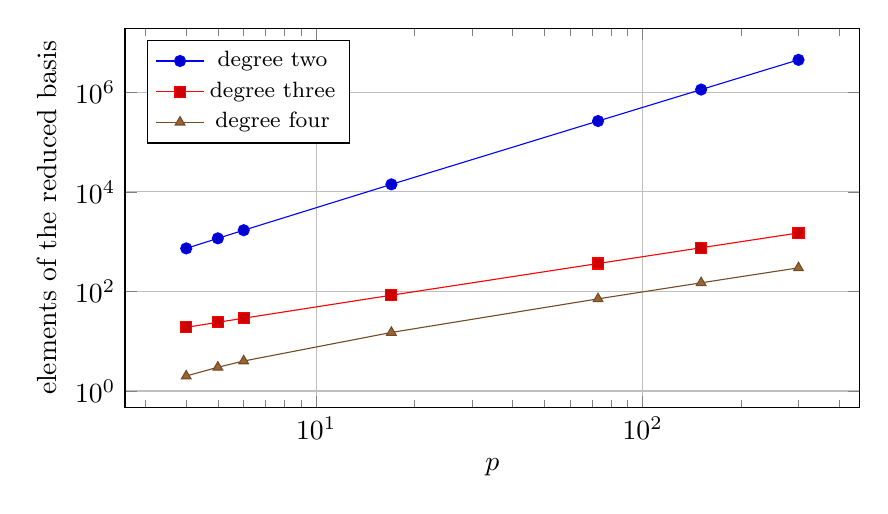
\begin{tikzpicture}\begin{axis}[width=0.9\linewidth, height=6.4cm, xmode=log, ymode=log, xlabel={$p$}, ylabel={elements of the reduced basis}, legend pos=north west, legend style={font=\footnotesize}, ymajorgrids, xmajorgrids]
\addplot+[mark=*] coordinates {(4,732) (5,1165) (6,1698) (17,14161) (73,265209) (151,1137483) (300,4494900)};
\addplot+[mark=square*] coordinates {(4,19) (5,24) (6,29) (17,84) (73,364) (151,754) (300,1499)};
\addplot+[mark=triangle*] coordinates {(4,2) (5,3) (6,4) (17,15) (73,71) (151,149) (300,298)};
\legend{degree two, degree three, degree four}\end{axis}\end{tikzpicture}
